 \documentclass[a4paper,12pt,final]{article}
\usepackage[english,francais]{babel}
\usepackage[utf8]{inputenc}
\usepackage[T1]{fontenc}
\usepackage[pdftex]{graphicx}
\usepackage{setspace}
\usepackage{hyperref}
\usepackage[french]{varioref}
\usepackage{sidecap}
\usepackage{array}
\usepackage{easytable}
\usepackage{listings}
\title{Rapport de stage}
\author{ABAK-KALI Nizar BAYASSI Majd}
\date{}

\newcommand{\reporttitle}{Rapport de CPS}     % Titre
\newcommand{\reportauthor}{ABAK-KALI Nizar \\ BAYASSI Majd} % Auteur
\newcommand{\numetudiant}{3402065 \\3402065}
\newcommand{\reportsubject}{Implementation d'un warcraft } % Sujet
\newcommand{\HRule}{\rule{\linewidth}{0.5mm}}
\setlength{\parskip}{1ex} % Espace entre les paragraphes



\hypersetup{
    pdftitle={\reporttitle},%
    pdfauthor={\reportauthor},%
    pdfsubject={\reportsubject},%
    %pdfkeywords={rapport} {vos} {mots} {clés}
}


\begin{document}

\begin{titlepage}

\begin{center}

\begin{minipage}[t]{0.48\textwidth}
  \begin{flushleft}
    
\includegraphics [width=30mm]{figures/url.png} \\[0.5cm]
    \begin{spacing}{1.5}
      \textsc{Université UPMC Paris VI}
    \end{spacing}
  \end{flushleft}
\end{minipage}


\textsc{\Large \reportsubject}\\[0.5cm]
\HRule \\[0.4cm]
{\huge \bfseries \reporttitle}\\[0.4cm]
\HRule \\[1.5cm]

\begin{minipage}[t]{0.3\textwidth}
  \begin{flushleft} \large
    \emph{Auteurs :}\\
    \reportauthor \\
    \emph{Numéros d'étudiants :}
    \numetudiant \\
  \end{flushleft}
\end{minipage}

\vfill


\end{center}

\end{titlepage}

\cleardoublepage

\tableofcontents
\sloppy

\cleardoublepage 

\part{Introduction}

\section{Enoncé}
	Ce projet consiste à développer un modèle, simplifié, avec
test embarqué du mode multi-joueur du jeu Warcraft:
Orcs and Humans TM , produit par Blizzard en 1994.
Dans cet épisode de la série, comme dans tout épisode de
cette série à l’innovation discutable, les joueurs dispensent
des ordres à gogo à leur chers sujets \− orcs ou humains \−
en appuyant et déplaçant furieusement leur main sur un
objet rond à boutons cliquables...

\section{Objectif du projet}
L’objectif du projet est multiple :
	\begin{itemize}
		\item[-] donner une spécification complète du modèle de jeu dans le langage de spécification vu en cours
		\item[-] réaliser à partir de la spécification une implémentation contractualisée, service et contrat sous
forme de tests embarqués, en utilisant le langage de votre choix comme par exemple le Java vu en
TME
		\item[-] définir à partir de la spécification des objectifs de test pour assurer les couvertures logiques, les paires de transitions, et une suite de scénarios utilisateurs
		\item[-]	réaliser à partir des objectifs de test une implémentation des cas de tests spécifiés, en Junit par
exemple
		\item[-] réaliser deux versions complètes du jeu, dont une totalement “buggée”. Ici, peu importe si les deux
réalisations sont avec interface graphique ou non. En revanche, elles doivent être en dehors de tout
modèle du jeu : pas de spécification, pas de contrats, pas de tests MBT
		 \item[-] recueillir les messages d’erreur lors de la confrontation de la version buggée avec les tests spécifiés.
	\end{itemize}



\cleardoublepage

\part{Organisation du Travail}

\section{Organisation du Projet}
Le projet est à  faire en binôme . Le projet ce compose de trois dossier : un dossier "src" qui contient les sources du projets , un dossier "spécifications"  qui contient les spécifications des services , et un dossier "doc" qui contient le rapport ainsi que le sujet du projet.\\
 Le dossier contenant les sources se découpe en les sous-dossier suivants : 
 	\begin{itemize}
 	\item services : qui contient les services coder en java .
 	\item implementations : contient les implémentations  des services .
 	\item decorators : contient les décorateurs implémentant les services .
 	\item contracts : contient les contrats héritant des décorateurs .
 	\item test : contient deux mains , un qui lance programme avec les contrats et un sans.
 	\item exceptions : contient les classes qui gèrent les exceptions du programme.
 	\end{itemize}
 	
 	Lors de la programmation nous nous y sommes pris par "étage" . C'est à dire, que nous avons d'abord écrit tout les services, puis  nous somme passer par par l’implémentation de ces services, ainsi de suites suivant l'ordre décrit ci-dessus .
 	

\section{Outils utilisés}

\subsection{Java et JUnit}
Nous avons programmer le jeu en Java et cela pour plusieurs raisons. Premièrement , les deux membres du binômes connaissent et maîtrise le langage.Deuxièmement,  nous avons été initié à la programmation par contrat en Java lors de nos travaux pratique. finalement, Java possèdes la librairie de teste JUnit très utiles pour pratiqué des testes unitaires .

\subsection{Communication et gestion de projet}
La communication au sain du groupe c'est principalement faite par mail et téléphone . La gestion du projet a été faite par Github. Ce choix et surtout dues au fait que l'outils qu'est Github est extrement pratique pour le travail en équipe et pour le télétravail .




\cleardoublepage

\part{Diagrammes}

Dans cette partie nous allons présenté les diagrammes représentant la composition du projet .

\section{Diagramme Use Case}
\begin{figure}[h]
	 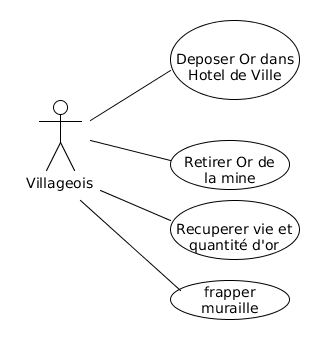
\includegraphics[scale=1]{figures/UseCaseVillageois.png}
	 \caption{Diagramme d'un cas d'utilisation d'un Villageois}
\end{figure}


\section{Diagramme de Classe}

\begin{figure}[h]
	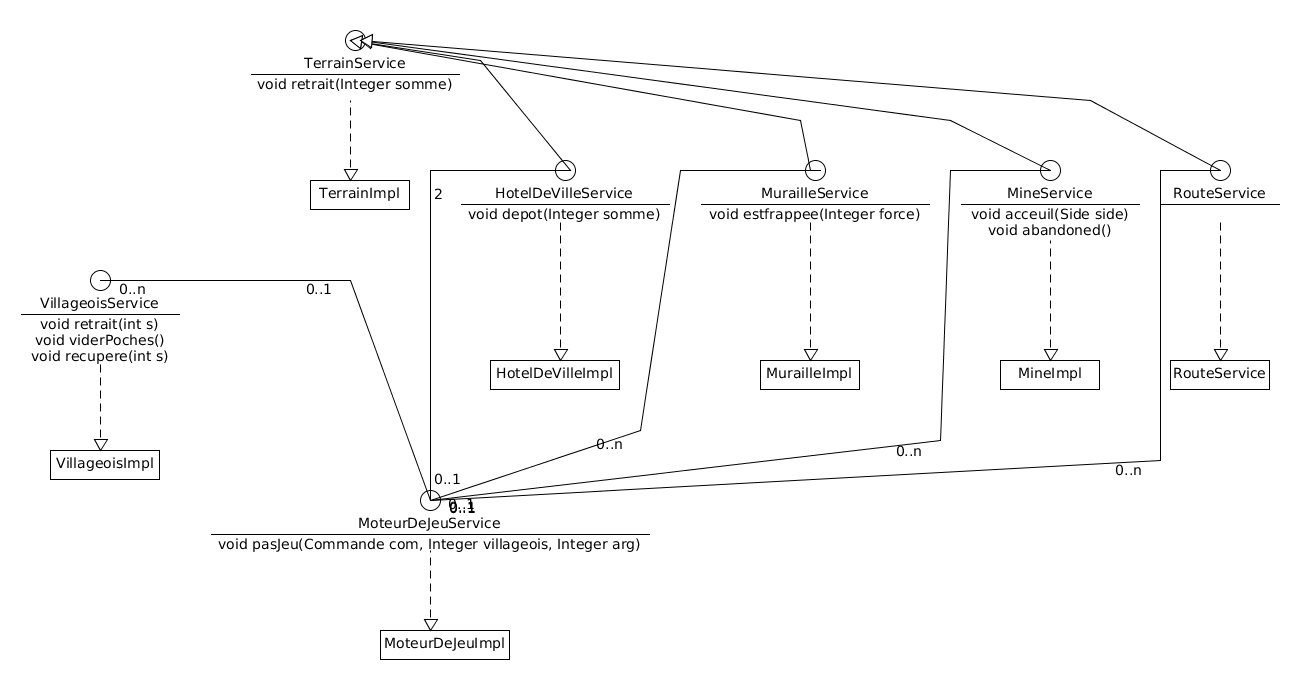
\includegraphics[scale=0.35]{figures/Diagramme_Classe.png}
	\caption{ Diagramme de Classe explicitant l'implémentation}
\end{figure}

\newpage

\section{Diagramme Composite}
	\begin{figure}[h]
	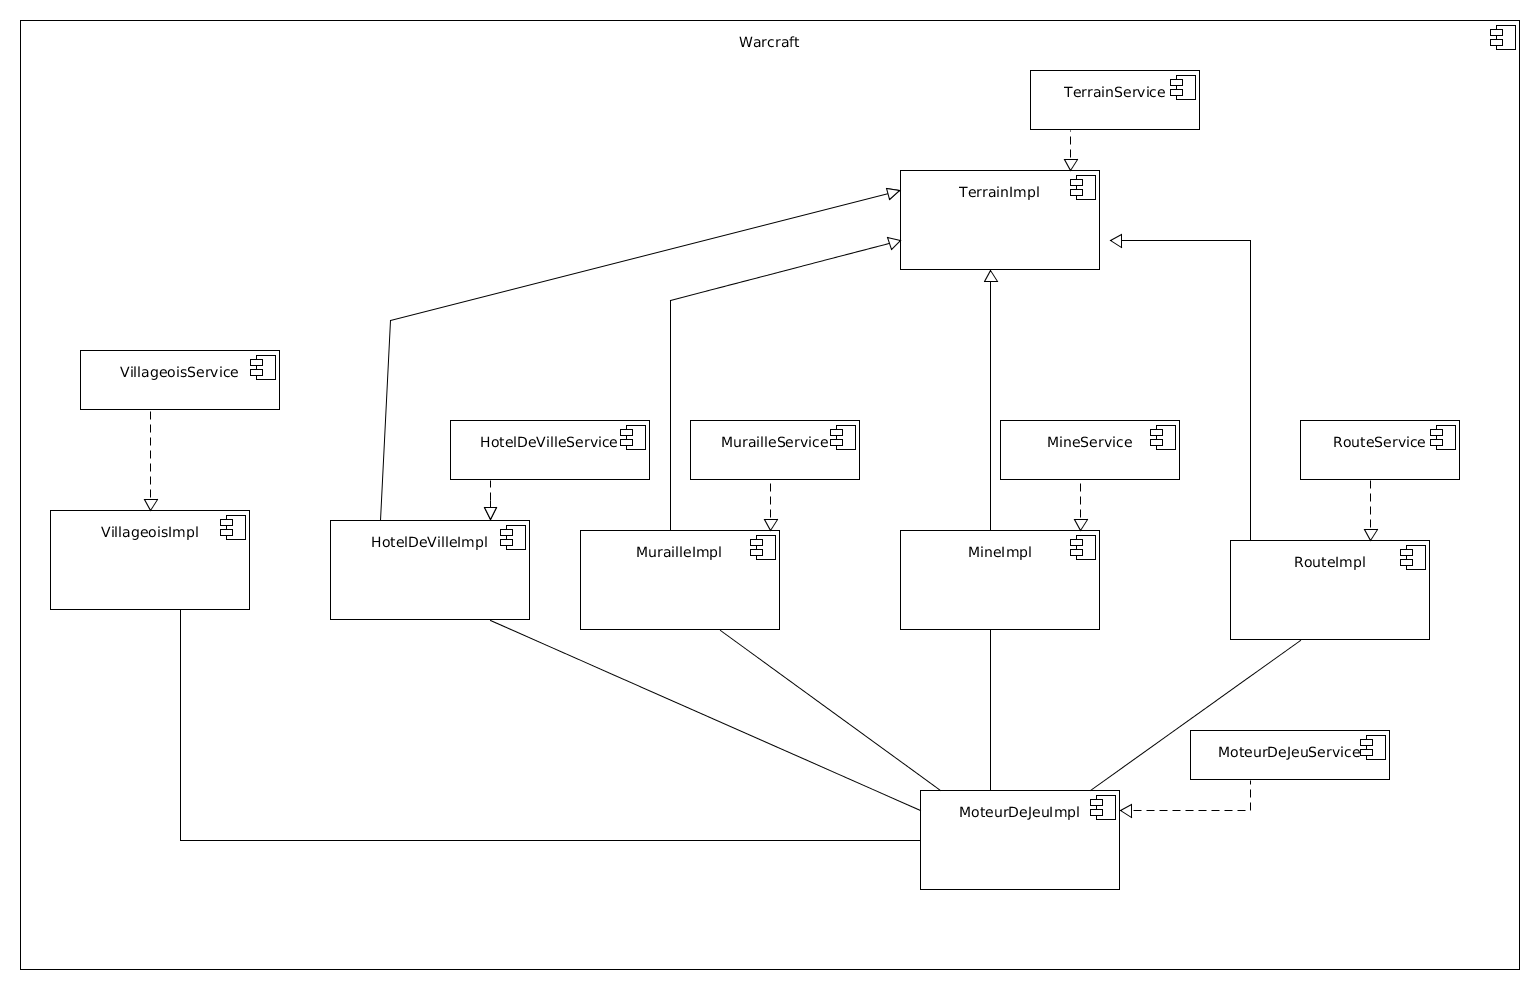
\includegraphics[scale=0.35]{figures/Diagramme_Composant.png}
	\caption{ Diagramme Composite}
\end{figure}

\cleardoublepage

\part{Problème et Solutions}

\section{Elaboration des Services}
Nous avons créer les services à partir des services donnée dans la correction du premier examen répartie. Bien sur plusieurs modification ont été apporté.
	\subsection{VillageoisService}
	Pour ce service nous avons ajouté les opérations "viderPoches" et "recupere".
	L'opération "viderPoches" a été ajouté afin qu'un villageois puisse vider sa quantité d'or dans l'hotel de ville .\\
	L'opération "recupere" permet comme son nom l'indique de recuperer des point de vie ainsi que de l'or .
	
	\subsection{TerrainService}
	Ce service a été ajouté afin de factoriser les caractéristiques qu'ont en commun les differentes structures du jeux , tel que : les mensurations , la quantité d'or restant , et un booléen pour indiquer si la structures est "laminé".
	
	

\section{Implementation des Services}

\section{Contrats}

\section{Testes}


\cleardoublepage

\part{Conclusion}
Ce projet avait pour but de nous initier à la programmation contractualisée mais aussi au plaisir d'être développeur de test .	
	Lors de ce projet  nous avons donné une spécification la plus complète possible du jeu dans le langage vue en cours disponible dans le dossier "spécification".
	Ensuite comme demandé nous avons réalisé à partir de la spécification  une implémentation contractualisée en utilisant le langage Java.
	Malheureusement , par manque de temps ,les test Junits sont manquant .
	 
	


\end{document}